\chapter{Architetture}

\section{Introduzione}

Il cuore di un software object-oriented si trova nel modello di dominio. Questo raccoglie i concetti estratti dall'analisi dei requisiti ed è composto da una rete di oggetti dotati di attributi e metodi che rispecchiano i \textit{dati} da memorizzare e le \textit{operazioni} necessarie alla loro elaborazione.
Questi elementi non dovrebbero avere al loro interno codice di supporto (finalizzato alla memorizzazione su un database, alla visualizzazione su interfaccia, all'invio su un canale ecc...), e in oltre questo non dovrebbe contenere frammenti di logica di dominio.
Il rischio altrimenti è quello di abbassare in maniera critica la manutenibilità del codice: le varie componenti sono accoppiate tra loro, e devono evolvere necessariamente in contemporanea.
Il test automatico diventa complesso, e si rischia di raggiungere presto lo stato di \textit{big ball of mud}\cite{microservices_architecture}.
Scrivere codice il più possibile disaccoppiato dalle tecnologie di contorno lo rende più manutenibile e testabile, ma d'altra parte può diminuire la produttività del team di sviluppo, soprattutto quando l'applicazione da sviluppare non è di eccessiva complessità.

Nel caso del lavoro corrente l'obiettivo è simulare l'evoluzione di un software da una versione monolitica ad una a microservizi: per far questo sono state sperimentate alcune architetture riconosciute, applicando quando possibile il principio di separazione delle responsabilità, fondamentale quando si parla di microservizi.

La prima architettura presa in esame è quella a livelli.

\section{Architettura a livelli}

Questo tipo di architettura è uno degli standard più affermati nello sviluppo di applicazioni enterprise.\\
Il codice è organizzato a livelli sovrapposti, ognuno dei quali può sfruttare i servizi esposti \textbf{soltanto} dai quelli sottostanti.
Esistono una serie di layers standard, di seguito se ne riportano alcuni dei più comuni\cite{ddd}:
\begin{itemize}
	\item Presentation: Fornisce informazioni e interpreta i comandi provenienti dall'esterno, in modo da interfacciarsi con un utente o un'altro software.
	\item Application: Sottile strato che dirige la logica di dominio delegando le azioni ai business objects.
	\item Model: Mantiene lo stato della logica di dominio e contiene le regole che la governano. \'E il cuore del software.
	\item Infrastructure: Fornisce funzionalità utili agli altri strati come persistenza, invio di messaggi, creazione interfaccia grafica ecc...
\end{itemize}
In questa visione il livello di business logic è consapevole dei livelli sottostanti, e può interagire direttamente con essi.
Dovendo gestire più ad alto livello la logica di dominio, per esempio aprendo e chiudendo una transazione, anche il livello application necessita di interagire con lo strato di infrastruttura.

Le linee guida per realizzare un'applicazione seguendo questa architettura prevedono di partizionare il codice in livelli coesi e dipendenti solamente da quelli sottostanti.

Esistono varie versioni di questa architettura, in cui i livelli di contorno variano: una di queste è la \textit{three layered architecture} (vedi figura \ref{fig:layered-architecture}), che prevede i livelli di \textit{Presentation} per la gestione della UI, \textit{Business Logic} per la logica di dominio e \textit{Persistence} per dialogare con i database.
Questi sono sufficienti per gran parte della applicazioni enterprise, in particolare se l'approccio usato è quello del monolite o del monolite a servizi.\\

\begin{figure}[h]
	\centering
	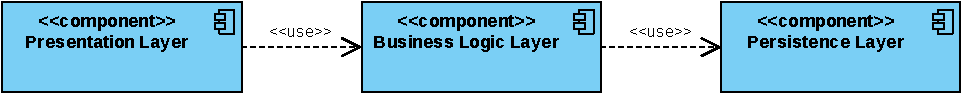
\includegraphics[width=\textwidth]{img/layered-architecture}
	\caption{Architettura a tre livelli}
	\label{fig:layered-architecture}
\end{figure}

Ogni livello può avere più istanze o essere ulteriormente separato, per esempio quando vi sono più interfacce grafiche verso la stessa applicazione, o più database che forniscono il servizio di persistenza.\\
Gli oggetti del modello di dominio devono essere, come già affermato, indipendenti dalle varie rappresentazioni, siano queste destinate ad UI, persistenza o altro.
Un indice di cattiva separazione delle responsabilità può essere per esempio la necessità di duplicare codice, o di modificare la logica di dominio quando si aggiunge una nuova interfaccia all'applicazione.\\
La separazione in layers permette inoltre di poter effettuare il rilascio delle varie parti dell'applicazione su macchine differenti, favorendone l'evoluzione e la scalabilità.
\section{Ports and adapters}

Una delle alternative all'architettura organizzata a \textit{layers} è l'architettura chiamata \textit{ports and adapters} o \textit{hexagonal architecture}\cite{microservices_architecture}.

\begin{figure}[h]
	\centering
	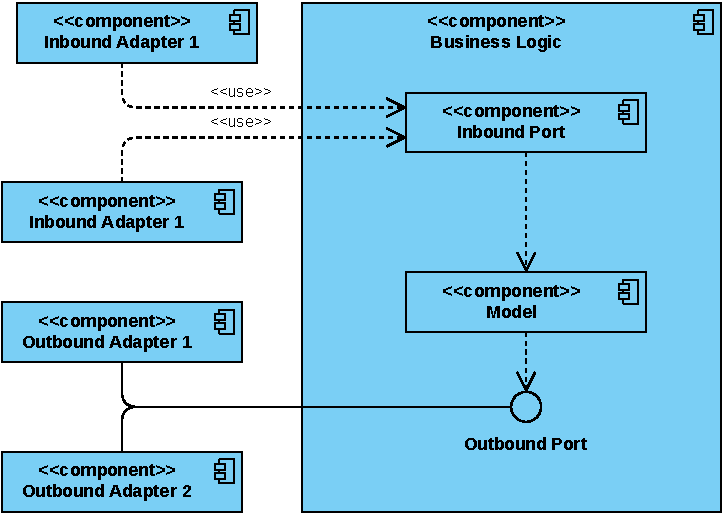
\includegraphics[width=\textwidth]{img/hexagonal-component-diagram}
	\caption{Architettura ports and adapters}
	\label{fig:hexagonal-architecture}
\end{figure}

Questo modo di organizzare i componenti del sistema è focalizzato sull'isolamento della logica di dominio.\\
Le comunicazioni di input/output con l'esterno sono guidate da interfacce \textbf{definite dal nucleo} e chiamate \textit{porte}: queste possono essere di tipo \textit{inbound} quando un modulo esterno ha necessità di invocare la logica di dominio, o di tipo \textit{outbound} quando il nucleo ha la necessità di invocare servizi esterni.
Ogni porta può avere più \textit{adattatori} associati, elementi che servono per collegare realmente i componenti esterni al nucleo.
La logica di dominio implementa le porte di tipo \textit{inbound}, che saranno usate dagli adattatori in ingresso per richiedere servizi all'applicativo.
Gli adattatori in uscita implementano le porte di tipo \textit{outbound}.

Partendo da un sistema costruito a livelli è possibile derivare l'equivalente in architettura esagonale considerando i seguenti fatti:
\begin{itemize}
	\item Se il client di un'applicazione a livelli è un'altro software, il livello di presentazione del primo può essere molto legato al livello di persistenza del secondo: ciò che è esterno alla logica di dominio quindi puòò essere visto semplicemente come un'interfaccia esterna
	\item In un'architettura a livelli moderna difficilmente la progettazione inizia dal livello di persistenza: spesso questo è realizzato da classi DAO (Data Access Object) che implementano un'interfaccia definita sulla base delle necessità del livello di business logic: questo crea una dipendenza in qualche modo inversa rispetto alla filosofia dell'architettura, enfatizzando il fatto che la logica di dominio è il centro dell'applicativo.
\end{itemize}

Rifattorizzare un progetto basato su architettura three tier per renderlo compatibile con quella ports/adapters a volte potrebbe limitarsi alla riorganizzazione dei package, senza necessitare modifiche al codice: questo perché i componenti di un'architettura a livelli spesso hanno un equivalente in architettura esagonale (vedi figura ).

Può capitare che data un'applicazione enterprise moderna
Anche in questo caso si cerca di rendere il più possibile indipendente il nucleo di un'applicazione dalle tecnologie di contorno, come database, sistema di scambio messaggi ecc...

Convertire un'applicazione service oriented realizzata a layers in una aderente all'architettura esagonale non è un'operazione complessa: se per esempio lo stack è di tipo 3-tier con una serie di servizi REST esposti che invocano internamente la logica di dominio ed uno strato di persistenza (es: JPA), il mapping è immediato (vedi figura \ref{fig:layered-hexagonal}).

\begin{figure}[h]
	\centering
	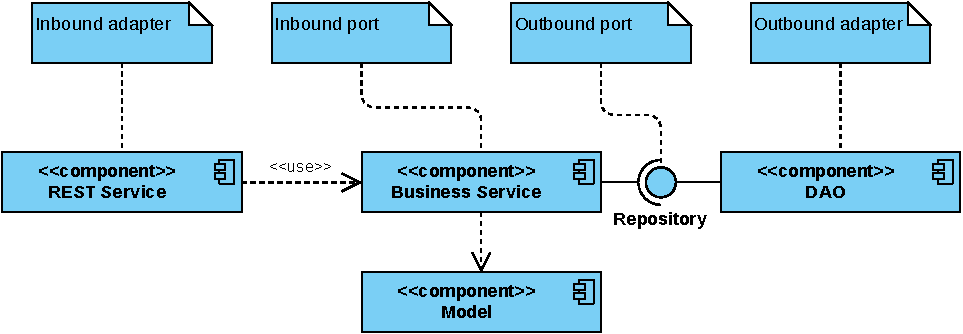
\includegraphics[width=\textwidth]{img/layered-hexagonal}
	\caption{Confronto architettura a livelli e ports/adapters}
	\label{fig:layered-hexagonal}
\end{figure}

I benefici di tale organizzazione diventano evidenti quando utilizzata all'interno di un software a microservizi, in quanto si è obbligati a identificare con chiarezza quali sono i confini del servizio, favorendo manutenibilità e testabilità.

\section{Logica di dominio}

Quando si parla di realizzare la logica di dominio per un'applicazione enterprise vi sono numerosi approcci che si possono adottare: di seguito riportiamo due patterns notevoli\cite{enterprise_app} che si contrappongono rispetto a dove verrà posta la maggior parte della logica.

\subsection{Transaction script}
La logica di dominio è posta principalmente in oggetti esterni al modello vero e proprio: il vero centro dell'applicazione è dato dai componenti chiamati \textit{Business Service} in figura \ref{fig:layered-hexagonal}.
L'idea è quella di avere entità più leggere, facilmente mappabili su un database.
Questo approccio può essere utile quando si utilizza un framework come JPA per la persistenza: si ha infatti il vantaggio di ridurre drasticamente il numero di righe di codice di tale livello, accettando il compromesso di "sporcare" le classi di modello con alcune annotazioni accoppiate ad una tecnologia.
Rendendo la separazione tra livelli o tra nucleo e porte più labile, questo approccio è adatto quando la logica di dominio non è particolarmente complessa e probabilmente non evolverà molto.

\subsection{Domain model}
La logica di dominio è contenuta quasi interamente all'interno degli oggetti del modello (\textit{Model} in figura \ref{fig:layered-hexagonal}).
Questo approccio permette di mettere in

\subsection{Architettura del software}
Il sistema è stato realizzato separando lo strato di UI da quello di business logic, realizzando secondo i principi dell'architettura \textit{ports/adapters}.\\
In particolare sono esposti verso l'esterno (inbound) una serie di servizi REST necessari all'interazione, ed è utilizzato un servizio di persistenza relazionale (outbound) necessario alla memorizzazione di informazioni come il profilo degli utenti, i progetti e le analisi effettuate.
In figura \ref{fig:architecture00} è mostrato lo schema generale.

\begin{figure}[h]
	\centering
	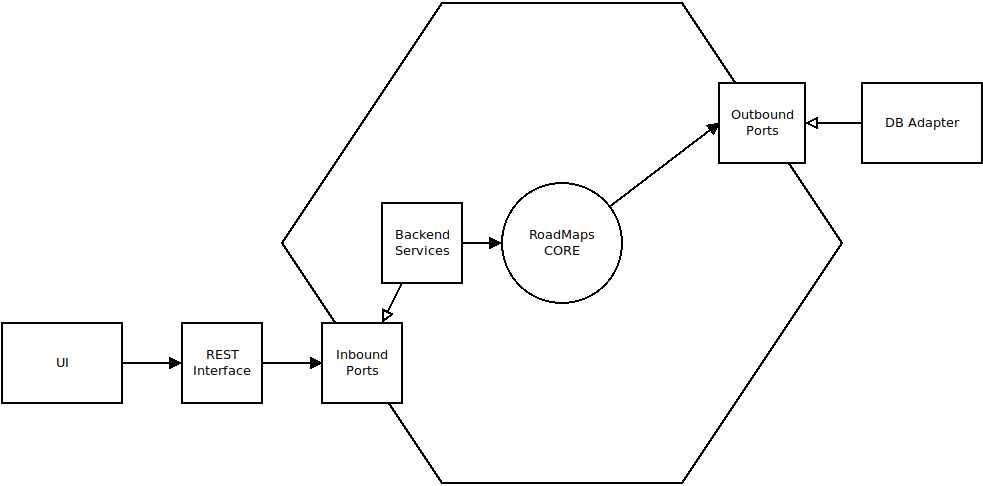
\includegraphics[width=\textwidth]{img/architecture00}
	\caption{Architettura generale}
	\label{fig:architecture00}
\end{figure}

I requisiti permettono di dividere naturalmente i servizi, le porte e gli adattatori in tre categorie:
\begin{itemize}
	\item Gestione degli utenti;
	\item Gestione delle configurazioni;
	\item Gestione dei progetti;
\end{itemize}

Un altro modulo piuttosto indipendente è quello relativo alla gestione delle analisi, ma essendo queste legate strettamente ad un progetto, saranno considerate parte dello stesso servizio.

Ognuno di questi moduli darà luogo ad un endpoint REST corrispondente ad uno o più casi d'uso, ad almeno un'entità principale e ad almeno una tabella su RDB.
Di seguito verrà riportata la descrizione di ognuno di questi blocchi partendo dal centro del modello di dominio e spostandosi all'esterno.

\subsubsection{Gestione degli utenti}
Il frammento di modello di dominio relativo alla gestione utenti è quello in figura \ref{fig:users_diagram}.

\begin{figure}[h]
	\centering
	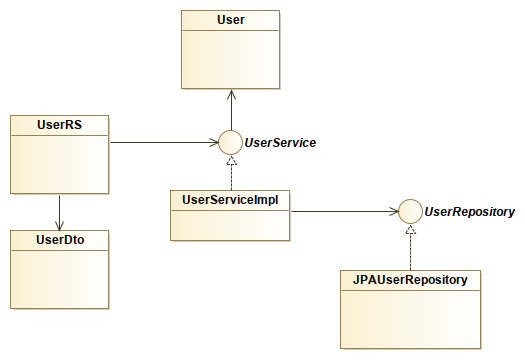
\includegraphics[width=\textwidth]{img/users_diagram}
	\caption{Diagramma delle classi relative alla gestione degli utenti}
	\label{fig:users_diagram}
\end{figure}

Dallo schema è possibile individuare quali siano le varie componenti associabili ai concetti dell'architettura esagonale:
\begin{itemize}
	\item UserService: Rappresenta una \textit{inbound port} che espone all'esterno le funzionalità relative ad un utente;
	\item UserServiceImpl: Implementa l'interfaccia \textit{UserService}, ed è quindi un \textit{inbound adapter};
	\item UserRepository: \'E una \textit{outbound port} necessaria per fornire alla logica di dominio le funzionalità di persistenza;
	\item JPAUserRepository: Implementazione di \textit{UserRepository} e quindi \textit{outbound adapter}, dipendente da una tecnologia specifica (Database relazionali + JPA), fornisce il collegamento con un RDBMS.
	\item UserRS: \'E un controller REST che espone verso il sottosistema UI i dati e le funzionalità di backend.
\end{itemize}

\subsubsection{Gestione delle configurazioni}
Il frammento di modello di dominio relativo alla gestione delle configurazioni è quello in figura \ref{fig:configurations_diagram}.

\begin{figure}[h]
	\centering
	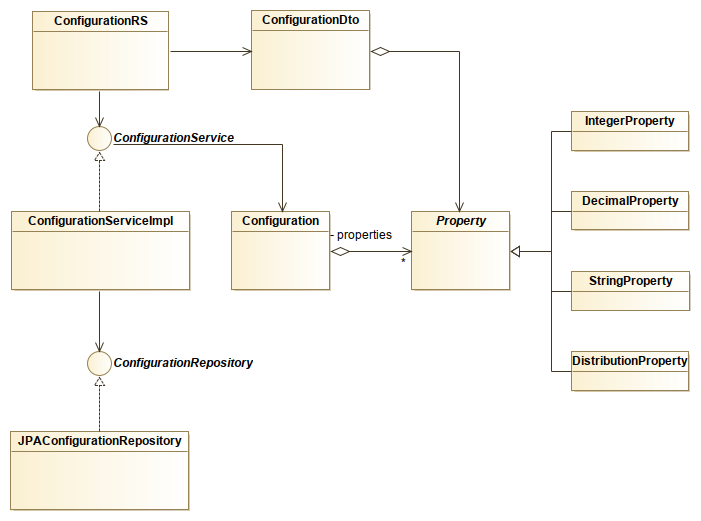
\includegraphics[width=\textwidth]{img/configurations_diagram}
	\caption{Diagramma delle classi relative alla gestione delle configurazioni}
	\label{fig:configurations_diagram}
\end{figure}

La struttura generale è equivalente a quella della sezione utenti: si hanno due interfacce \textit{ConfigurationService} e \textit{ConfigurationRepository} corrispondenti alle porte \textit{inbound} e \textit{outbound}, con i relativi adattatori \textit{ConfigurationServiceImpl} e \textit{JPAConfigurationRepository}.\\
Vi è sempre un controller REST per ricevere comandi dall'esterno del sistema, utilizzando in questo caso direttamente alcune entità del modello di dominio.

\subsubsection{Gestione dei progetti}
Il frammento di modello di dominio relativo alla gestione utenti è quello in figura \ref{fig:projects_diagram}.

\begin{figure}[h]
	\centering
	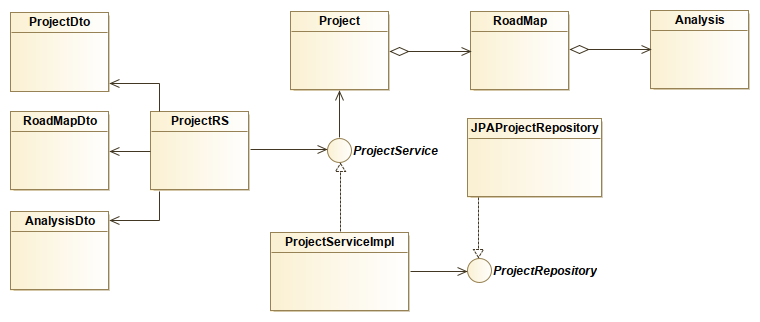
\includegraphics[width=\textwidth]{img/projects_diagram}
	\caption{Diagramma delle classi relative alla gestione dei progetti}
	\label{fig:projects_diagram}
\end{figure}

Anche in questo caso vi sono le stesse porte e adattatori più il controller REST relativo.
